\documentclass[11pt]{article}

\usepackage[utf8]{inputenc}
\usepackage[margin=2.5cm]{geometry}
\usepackage{enumerate}
\usepackage{listings}
\usepackage{color}
\usepackage[hidelinks]{hyperref}
\usepackage{csquotes}
\usepackage{graphicx}
\usepackage{amsmath}
\DeclareGraphicsExtensions{.png}

\setlength\parindent{0pt}
\setcounter{section}{3}

\definecolor{pblue}{rgb}{0.13,0.13,1}
\definecolor{pgreen}{rgb}{0,0.5,0}
\definecolor{pred}{rgb}{0.9,0,0}
\definecolor{pgrey}{rgb}{0.46,0.45,0.48}

\lstset{
	language=Java,
	tabsize=2,
	showspaces=false,
	showtabs=false,
	breaklines=true,
	showstringspaces=false,
	breakatwhitespace=true,
	commentstyle=\color{pgreen},
	keywordstyle=\color{pblue},
	stringstyle=\color{pred},
	basicstyle=\small\ttfamily,
	numbers=left,
	numberstyle=\tiny,
	numbersep=5pt
}

\title{Distributed Systems HS 2016\\Assignment 3}
\author{Markus Hauptner, Johannes Beck, Linus Fessler}
\date{\today}

\begin{document}
\maketitle

\section{Mini-Test}

\begin{enumerate}

\item {What are the main advantages of using Vector Clocks over Lamport timestamps?}
 
The main advantage of Vector Clocks over Lamport timestamps is that with Vector Clocks, any process in a distributed system knows the causal dependencies of events. This holds because Vector Clocks fulfill the strong clock condition defined as follows:

Let $e_1,e_2$ be events. Let $C(e)$ denote the Vector Clock of event $e$. Then $$e_1 \prec e_2 \Longleftrightarrow C(e_1) < C(e_2)$$ (where $\prec$ is the "happens before" relation between events and the $<$ relation as defined in question 2).

Even if the strong clock condition is not required, Vector Clocks have the advantage that they are unique. Two different events can have the same Lamport timestamp but not the same time vector.

\item {Give the two conditions for two Vector Clocks to be causally dependent?}

(Remark: The notion of "causal dependence" for Vector Clocks was not defined in class/in the exercise slides. So we assume that we have to give the conditions for the $<$ relation.)\\
Let $C,D$ be Vector Clocks in a system with $n$ processes. Let $C_i$ denote the i-th element of $C$. Then $C < D$ if and only if:
\begin{enumerate}
\item $C \not= D$ and
\item $C_i \le D_i ~|~\forall i : 1 \le i \le n$.
\end{enumerate}


\item {Does a clock tick happen before or after the sending of a message. What are the implications of changing this?}

The clock ticks happen before the sending of a message. If the tick happened after sending the message, the clock condition would not be fulfilled. Consider the following situation: 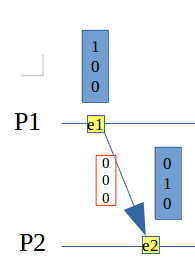
\includegraphics[scale=0.4]{question3_example}

In this case, the clock condition is violated because clearly $$e1 \prec e2 \wedge C(e1) = \begin{pmatrix} 1 \\ 0 \\ 0 \end{pmatrix} \not< \begin{pmatrix} 0 \\ 1 \\ 0 \end{pmatrix} = C(e2).$$
 
\item {Fill in the corresponding vector clocks from Figure 1.}

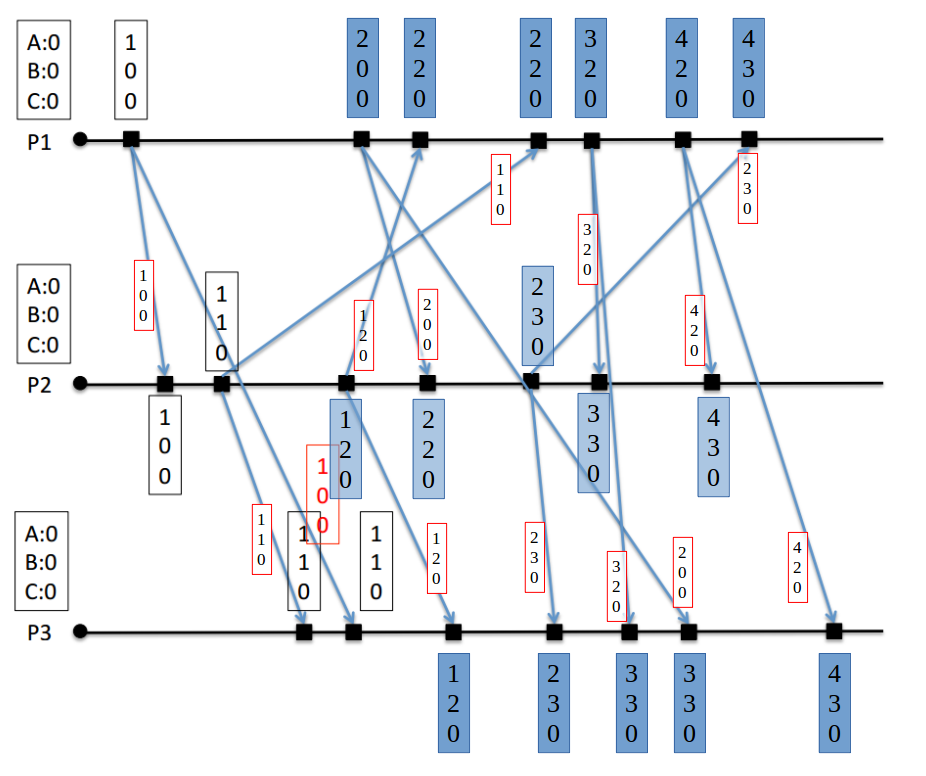
\includegraphics[scale=0.4]{figure1_completed}
\item {Read the paper \textit{Dynamic Vector Clocks for Consistent Ordering of Events in Dynamic Distributed Applications} by Tobias Landes that gives a good overview on the discussed methods. In particular, which problem of vector clocks is solved in the paper?}

In a system with "normal" vector clocks every process has to know the total number of processes in advance. This number has to be constant and cannot change.
The paper introduces the concept of dynamic vector clocks which can be used in systems with a varying number of processes.
\end{enumerate}

\end{document}
